\documentclass[a4paper,12pt]{article}
\usepackage[utf8x]{inputenc}
\usepackage[T1]{fontenc}

%\usepackage[T2A]{fontenc} % jei yra kirilica
\usepackage[hmargin={30mm,15mm},vmargin={20mm,20mm},bindingoffset=0mm]{geometry}
\usepackage[onehalfspacing]{setspace}
\usepackage[colorlinks=true, linkcolor=blue, citecolor=blue, urlcolor=blue, unicode]{hyperref}

%\parindent=7mm
\renewcommand{\refname}{Literatūros sąrašas} % article
%\renewcommand{\bibname}{Literatūros sąrašas} % report
\renewcommand{\contentsname}{Turinys}
\usepackage[T1]{fontenc} 

% Lukas paketai
\usepackage{graphicx}
\usepackage{indentfirst}
\usepackage{setspace}
\usepackage{placeins}
\usepackage{booktabs}% http://ctan.org/pkg/booktabs
\usepackage{tabularx}% http://ctan.org/pkg/tabularx
\usepackage[parfill]{parskip}
\usepackage[unicode]{hyperref}
\usepackage{hyperref}
\usepackage{tocloft}
\usepackage{graphicx}
\newcommand\AtPageUpperRight[1]{\AtPageUpperLeft{%
   \makebox[\paperwidth][r]{#1}}}
\usepackage[dotinlabels]{titletoc}
\usepackage[capposition=top]{floatrow}
\hypersetup{
    colorlinks,
    citecolor=black,
    filecolor=black,
    linkcolor=black,
    urlcolor=black
}
\usepackage{secdot}




\begin{document}
\graphicspath{ {/} }

\renewcommand{\cftdot}{.}	
\renewcommand{\cftsecleader}{\cftdotfill{\cftdotsep}}

\thispagestyle{empty} % nerasomas psl. nr


\begin{center}
 VILNIAUS UNIVERSITETAS 
 
MATEMATIKOS IR INFORMATIKOS FAKULTETAS

MATEMATINĖS INFORMATIKOS KATEDRA

\vspace{4cm}

Projekto vadovė \ \ \textbf{Lukas Tutkus} \\
\textbf{Julius Daukšas} \\
\textbf{Dominykas Smaliukas} \\
\textbf{Robert Stankevič} \\

\vspace{0.2cm}

Bioinformatikos studijų programos grupė BioSawmill



\vspace{3cm}
\textbf{\Large Dvimatė pjovimo optimizacija}\\
\textbf{\Large Projekto planas}

\vfill

Vilnius \ \  2015
\end{center}



\clearpage

\tableofcontents
\clearpage
\section{Funkciniai ir nefunkciniai reikalavimai}
\begin{frame}
\centering

\label{my-label}
\begin{tabular}{|l|l|l|}
\hline
\textbf{ID}	& \textbf{Reikalavimai}						& \textbf{Moduliai}  \\ \hline

F1	& Registracija										& 1	     		\\ \hline

F2	& Prisijungimas prie sistemos						& 1, 3			\\ \hline

F3	& Atsijungimo nuo sistemos							& 1, 3			\\ \hline

F4	& Slaptažodžio atgavimas								& 1, 3			\\ \hline

F5	& Paskyros parametrų keitimas 	  					& 1, 3			\\ \hline 

F6	& Vartotojo paskyros ištrinimas						& 1, 3			\\ \hline

F7	& Vartotojo paskyros atgavimas						& 3				\\ \hline

F8	& Pjovimo optimizacijos duomenų įvedimas				& 1, 3			\\ \hline

F9	& Pjūvio plano optimizavimas           	   			& 2				\\ \hline

F10	& Optimizuotų pjūvio planų informacijos pateikimas	& 2     			\\ \hline

F11	& Optimizuotų pjūvio planų variantų pasirinkimas		& 1, 3			\\ \hline

F12 & Pjūvio plano ruošinio atsisiuntimas				& 1, 3			\\ \hline

F13 	& Pjūvio plano informacijos išsaugojimas				& 1, 3			\\ \hline

F14	& Kalbos pasirinkimas(LT, EN)						& 1, 3			\\ \hline

NF1 & Užtikrinti kalbos pakeitimą						& 1, 3			\\ \hline

NF2 & Slaptažodžio ilgis didesnis už 8					& 1, 3			\\ \hline 

NF3 & Prisijungimo duomenys išskyrus slaptažodį-unikalūs	& 1, 3			\\ \hline 

NF3 & 
\begin{tabular}[c]{@{}l@{}}
Prisijungime pakeičiamai dalyvauja vartotojo vardas\\
ir el.paštas(bent vienas turi atitikti varotojo įrašą).			
\end{tabular}											& 1, 3			\\ \hline 
\end{tabular}
\end{frame}

\vspace{1cm}
\textbf{Moduliai} \\
1-Varotojų, 2- P.O, 3 - Administratoriaus.


\vspace{1cm}
informacija - panelių kiekis, bendras jų plotas, likutis, detalių išdėstymas.

\section{Atsekamumo lentelė}
\begin{frame}
\centering
\hspace{-1cm}
\label{my-label}
\begin{tabular}{|l|c|}
\hline
\textbf{Užsakovo poreikiai}						& \textbf{Reikalavimai} 		\\ \hline

\begin{tabular}[c]{@{}l@{}}
Vartotojas nurodo reikalingų detalių ilgius (mm), 
aukščius (mm) ir kiekius.                                                                                                                                                                                                                                                                              
\end{tabular} 									& F8	                 		\\ \hline

\begin{tabular}[c]{@{}l@{}}
Sistema optimizuoja detalių išpjovimą iš standartinių panelių 1200x2500.\\ 
Po to pakartoja šį procesą su standartiniais paneliais 1200x3050.\\ 
(Turėkite omenyje, kad pjovimo plotis yra 4 mm, todėl iš standartinės \\ 
panelės 1200x2500 negalima išpjauti 2 detalių 600x2500.)
\end{tabular}									& F9, F10					\\ \hline

\begin{tabular}[c]{@{}l@{}}
Sistema pateikia abiejų variantų informaciją vartotojui ir pasirenka, \\ 
kuris variantas jam labiau tinka. Vartotojui pasirinkus, sistema \\ 
turi parodyti ekrane pjovimo planą su galimybe jį atsispausdinti \\
(su atspausdintu planu vartotojas gali kreiptis į tiekėją, kad \\ 
išpjautų jam reikiamas detales).
\end{tabular}									& F11, F12	 				\\ \hline

Planuojama sistemą pateikti kaip paslaugą išoriniams vartotojams.                                                                                                                                                                                                                                                                                         												& F1, F2	, F3, F4, F5, F6		\\ \hline

Įvedami standartinių panelių dydžiai.			& F8							\\ \hline

\end{tabular}
\end{frame}


\section{Klasių diagramos}

\section{Naudojimo atvejų aprašai(Use-cases)}

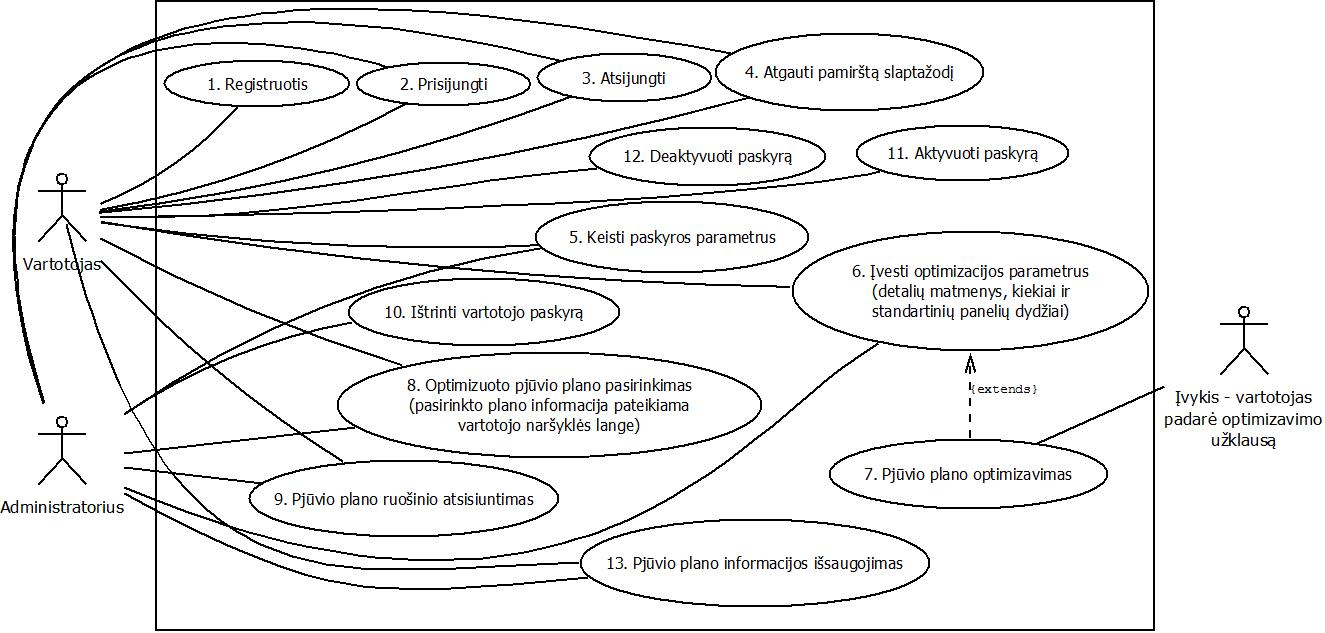
\includegraphics[width=18cm, height=10cm]{diagrama}


\begin{frame}
\centering
\hspace{-1cm}
\label{my-label}
\begin{tabular}{|l|l|}
\hline
\textbf{Pavadinimas}  		& Registracija 							\\ \hline
\textbf{Dalyviai}  			& Vartotojas								\\ \hline
\textbf{Paskirtis}  			& Sukurti naujo vartotojo paskyrą		\\ \hline
\textbf{Kritiškumas}			& Būtinas 								\\ \hline
\textbf{Pradinės sąlygos}   	& Atidaryti tinklapy naršyklėje			\\ \hline
\textbf{Rezultatas}   		& Sistemos duomenų bazėje sukurtas 
							naujo vartotojo įrašą,vartotojas					\\ \hline
\textbf{
	\begin{tabular}[c]{@{}l@{}}
		Tipinė eiga ir kiti\\ 
		galimi variantai
	\end{tabular}
} &   
\begin{tabular}[c]{@{}l@{}}
	1. Vartotojas atidaręs P.O. tinklapy prieš naudojantis juo turi prisiregistruoti.\\
	Visų pirmą registravimosi formoje turi užpildyti	privalomus laukus: \\
	Unikalų vartotojo vardą ir unikalų, galiojantį el.paštą, slaptažodį.\\\\
	
	2. Suvedus duomenis paspausti mygtuką.\\\\
	
	3. Jeigu suvestas vartotojo vardas, bei paštas unikalus duomenų bazėje,\\
	tada sukuriamas vartotojo įrašas duomenų bazėje ir vartotojas\\
	nukreipiamas į jo naujos paskyros langą. \\
	Kitu atveju vartotojui pranešama, kad reikia įvesti iš naujo, \\
	nes suvestas paštas ir ar vardas pasikartojo.
\end{tabular} \\ \hline

\end{tabular}
\end{frame}

% <<<<<<<<<<<<<<<<<<<<<<<<<<<<<

\vspace{2cm}

\begin{frame}
\centering
\hspace{-1cm}
\label{my-label}
\begin{tabular}{|l|l|}
\hline
\textbf{Pavadinimas}  		&	Prisijungimas prie sistemos						\\ \hline
\textbf{Dalyviai}  			&	Vartotojas, administratorius						\\ \hline
\textbf{Paskirtis}  			&	Prieiga prie vartotojo paskyros, P.O. 			\\ \hline
\textbf{Kritiškumas} 		&	Būtinas											\\ \hline
\textbf{Pradinės sąlygos}	&	Naudotojo įrašas sistemos duomenų bazėje			\\ \hline
\textbf{Rezultatas}			&  	Prieiga prie savo paskyros bei P.O. atlikimas	\\ \hline
\textbf{
	\begin{tabular}[c]{@{}l@{}}
		Tipinė eiga ir kiti\\ galimi variantai
	\end{tabular}} 				&   
\begin{tabular}[c]{@{}l@{}}
1. Prisijungimo lange suvesti prisijungimo duomenis:\\ 
vartotojo vardą arba paštą ir slaptažodį.\\\\

2. Paspausti prisijungimo mygtuką.\\\\

3. Sistema patikrina ar prisijungimo duomenys atitinka naudotojo įrašo\\
duomenis(vardą ar paštą ir slaptažodį) duomenų bazėje.\\
Naudotojas nukreipiamas į savo paskyrą jei įvesti duomenys atitiko.\\
Kitu atveju pranešama, jog prisijungimo duomenys klaidingi,\\
lieka bandyti dar 2 kartus prisijungti iš naujo.\\\\

4. Atsiranda mygtukas "Istorija", sąrašas išsaugotų P.O.\\
Paspaudus pavadinimą atsiranda išsaugotą informaciją.\\
\end{tabular} \\ \hline

\end{tabular}
\end{frame}

% <<<<<<<<<<<<<<<<<<<<<<<<<<<<<
\vspace{1cm}
\begin{frame}
\centering
\hspace{-1cm}
\label{my-label}
\begin{tabular}{|l|l|}
\hline
\textbf{Pavadinimas}			&	Atsijungimas nuo sistemos 					\\ \hline
\textbf{Dalyviai}			&   Vartotojas, administratorius    				\\ \hline
\textbf{Paskirtis}			&  	Nutraukti sistemos naudojimosi sesiją       	\\ \hline
\textbf{Kritiškumas}			&  	Vidutinis									\\ \hline
\textbf{Pradinės sąlygos}	& 	Sistemos naudotojas yra prisijungęs 
								prie sistemos   								\\ \hline
\textbf{Rezultatas}			&	Nutraukta sistemos naudotojo sesija      
\\ \hline
\textbf{
\begin{tabular}[c]{@{}l@{}}
	Tipinė eiga ir kiti\\ 
	galimi variantai
\end{tabular}} &
\begin{tabular}[c]{@{}l@{}}
	1. Sistemos naudotojas paspaudžia atsijungimo mygtuką, \\
	jo sesija sustabdoma.
\end{tabular} \\ \hline
\end{tabular}
\end{frame}

% <<<<<<<<<<<<<<<<<<<<<<<<<<<<<

\vspace{1cm}
\begin{frame}
\centering
\hspace{-1cm}
\label{my-label}
\begin{tabular}{|l|l|}
\hline
\textbf{Pavadinimas}			&  	Slaptažodžio atgavimas					\\ \hline
\textbf{Dalyviai}			&	Vartotojas, administratorius				\\ \hline
\textbf{Paskirtis}			&   Sužinoti pamirštą slaptažodį.			\\ \hline
\textbf{Kritiškumas}			&	Būtinas 									\\ \hline
\textbf{Pradinės sąlygos}	&  								 			\\ \hline
\textbf{Rezultatas}			&	\begin{tabular}[c]{@{}l@{}}
								Naudotojas į el. paštą gauna savo \\
								slaptažodžio priminimą
								\end{tabular}   						\\ \hline
\textbf{
	\begin{tabular}[c]{@{}l@{}}
		Tipinė eiga ir kiti\\ 
		galimi variantai
	\end{tabular}
} &   
\begin{tabular}[c]{@{}l@{}}

	1. Paspaudžiamas pamiršto slaptažodžio atgavimo mygtukas.\\\\
	
	2. Atsidariusioje formoje nurodomas el. paštas\\ 
	ar vardas, kurie yra užregistruoti sistemoje.\\\\
	 
	3. Paspaudžiamas mygtukas ir vykdoma forma. \\\\
	
	4. Jei el. paštas ar vardas egzistuoja sistemos duomenų bazėje, tada bus\\ 
	nusiunčiamas laiškas su slaptažodžiu į naudotojo įraše esantį paštą . \\

	Jei nei vardo, nei el. pašto atitikmens nerandama \\
	duomenų bazėje, perspėjama, kad įvesti duomenys klaidingi \\
	ir pasiūloma prisiregistruoti.
\end{tabular} \\ \hline

\end{tabular}
\end{frame}

% <<<<<<<<<<<<<<<<<<<<<<<<<<<<<
\vspace{1cm}
\begin{frame}
\centering
\hspace{-1cm}
\label{my-label}
\begin{tabular}{|l|l|}
\hline
\textbf{Pavadinimas}			&  	Paskyros parametrų keitimas						\\ \hline
\textbf{Dalyviai}			&	Vartotojas, administratorius						\\ \hline
\textbf{Paskirtis}			&	Leisti pakeisti paskyros duomenis				\\ \hline
\textbf{Kritiškumas}			& 	Vidutinis										\\ \hline
\textbf{Pradinės sąlygos}	&  	Įykdytas prisijungimas							\\ \hline
\textbf{Rezultatas}			&   Pakeista paskyros informacija					\\ \hline
\textbf{
	\begin{tabular}[c]{@{}l@{}}
		Tipinė eiga ir kiti\\
		galimi variantai
	\end{tabular}
} &   
\begin{tabular}[c]{@{}l@{}} 
	1. Spaudžiamas paskyros redagavimo mygtukas.\\\\
	
	2. Vartotojas gali pakeisti norimus paskyros duomenis.\\
	Administratorius gali pakeisti bet kurios paskyros \\
	prisijungimo vardą, prisijungimo paštą ir tik savo \\
	paskyros slaptažodį.\\\\
	
	3. Spaudžiamas pakeitimų išsaugojimo mygtukas.\\\\
	
	4. Pakeitimai turi atitikti registracijos formos reikalavimus \\
	Prisijungimo vardas, paštas netuščias, slaptažodis iš 8 \\
	ar daugiau simbolių. \\
	Atitikus reikalavimus pakeitimai išsaugomi paskyroje, duomenų bazėje \\
	ir administratoriaus matomų paskyrų saraše jei keistas ne slaptažodis.\\
	Neatitikus pažymimi neleistinas reikšmes įgiję laukai.\\

\end{tabular}																	 \\ \hline

\end{tabular}
\end{frame}

% <<<<<<<<<<<<<<<<<<<<<<<<<<<<
\vspace{1cm}
\begin{frame}
\centering
\hspace{-1cm}
\label{my-label}
\begin{tabular}{|l|l|}
\hline
\textbf{Pavadinimas}			&  	Vartotojo paskyros ištrinimas.						\\ \hline
\textbf{Dalyviai}			&	Vartotojas, administratorius						\\ \hline
\textbf{Paskirtis}			&	Ištrinti nenaudojamas ar kenkėjiškas paskyras	\\ \hline
\textbf{Kritiškumas}			& 	Būtinas											\\ \hline
\textbf{Pradinės sąlygos}	& 	Įykdytas prisijungimas							\\ \hline
\textbf{Rezultatas}			&   Ištrintas tam tikras vartotojo įrašas        	\\ \hline
\textbf{
	\begin{tabular}[c]{@{}l@{}}
		Tipinė eiga ir kiti\\ 
		galimi variantai
	\end{tabular}
} &   
\begin{tabular}[c]{@{}l@{}} 
	1.	Vartotojui pateikiamas savo paskyros trinimo mygtukas.\\
	Administratorius turi paskyrų sarašą, kur yra visos išskyrus\\
	jo pačio paskyros. Saraše laikomi vartotojų vardai bei paštai.\\ 
	Paspaudus ant tam tikros paskyros iškyla tos paskyros trinimo myguktas.\\\\
	
	2. 	Spaudžiamas paskyros trinimo mygtukas.\\\\

	3.	Vartotojas tai paspaudęs yra atjungiamas nuo sistemos,\\
	o jo paskyra sunaikinama. \\
	Administratoriui paspaudus trinimo mygtuką tam tikra paskyrą \\
	ištrinama iš duomenų bazės bei iš paskyrų sarašo.\\
	Ištrintos paskyros vardas, paštas irašomi į ištrintų paskyrų sąraša.\\
\end{tabular} \\ \hline

\end{tabular}
\end{frame}

% <<<<<<<<<<<<<<<<<<<<<<<<<<<<<
\vspace{1cm}
\begin{frame}
\centering
\hspace{-1cm}
\label{my-label}
\begin{tabular}{|l|l|}
\hline
\textbf{Pavadinimas}			&  	Vartotojo paskyros atgavimas						\\ \hline
\textbf{Dalyviai}			&	Administratorius									\\ \hline
\textbf{Paskirtis}			&	Atgauti reikalingas paskyras						\\ \hline
\textbf{Kritiškumas}			& 	Būtinas											\\ \hline
\textbf{Pradinės sąlygos}	& 	Ištrinta bent viena vartotojo paskyrą			\\ \hline
\textbf{Rezultatas}			&   Ištrintas vartotojo įrašas yra gražinamas       	\\ \hline
\textbf{
	\begin{tabular}[c]{@{}l@{}}
		Tipinė eiga ir kiti\\ 
		galimi variantai
	\end{tabular}
} &   
\begin{tabular}[c]{@{}l@{}} 
	1.	Administratoriui pateikiamas ištrintų vartotojo paskyrų sąrašas, \\
	kuriame matomas vartotojo vardas, paštas.\\
	Paspaudus ant tam tikros paskyros iškyla tos paskyros atgavimo\\
	mygtukas.\\\\
	
	2. 	Spaudžimas vartotojo paskyros atgavimo mygtukas.\\\\
	
	3. 	Paskyra sunaikinama ištrintų paskyrų saraše, \\
	į jos paštą nusiunčiamas laikinas(1 sav.) prisijungimo slaptažodis.\\
	Paskyra įrašoma į administratoriui matomų paskyrų sąrašą tik tada\\ 
	kai patvirtinama į paštą nusiūsta nuoroda. \\


\end{tabular} \\ \hline

\end{tabular}
\end{frame}

% <<<<<<<<<<<<<<<<<<<<<<<<<<<<<

\vspace{1cm}
\begin{frame}
\centering
\hspace{-1cm}
\label{my-label}
\begin{tabular}{|l|l|}
\hline
\textbf{Pavadinimas}			&  	Pjovimo optimizacijos duomenų įvedimas.						\\ \hline
\textbf{Dalyviai}			&  	Vartotojas, administratorius  									\\ \hline
\textbf{Paskirtis}			&  	\begin{tabular}[c]{@{}l@{}}
									Parametrų perdavimas, pagal kuriuos algoritmas optimizuos detales \\
									ant standartinių  panelių
								\end{tabular}									\\ \hline
\textbf{Kritiškumas}			& 	Būtinas											\\ \hline
\textbf{Pradinės sąlygos}	& 	Naudotojas yra prisijungęs ir atsidaręs pjovimo optimizavimui skirtą formą \\ \hline
\textbf{Rezultatas}			& 	\begin{tabular}[c]{@{}l@{}}
									Įvesti reikalingus parametrus optimizacijos vykdymui. \\
								\end{tabular} \\ \hline
\textbf{
	\begin{tabular}[c]{@{}l@{}}
		Tipinė eiga ir kiti\\ galimi variantai
	\end{tabular}
} &   
\begin{tabular}[c]{@{}l@{}} 
	1. Optimizacijos formoje suteikiami pasirenkami standartiniai panelių \\
	dydžiai(1200x2500, 1200x3050), prie jų galima įvesti\\
	panelių	matmenis. Optimizacija galės vykti tik tada kai bus nurodyta ar \\
	įvesta bent viena panelė.\\\\
	
	2. Taip pat nurodomi reikalingų detalių:\\
		ilgiai (mm),	 aukščiai (mm) ir kiekiai.\\
	Taip pat galima įkelti xlsx formato failą, su ilgio, aukščio stulpeliais.\\\\
	
	3. Detalių duomenys nurodomi sveikaisiais skaičiais, jų kiekis \\
	ne didesnis už 1000. Ilgiai, aukščiai mažesni ar lygūs\\
	nurodytom standartinėm panelėm. Standartinės panelės matmenys \\
	galimi nuo 10mm iki 20000mm, kiekis 10. \\\\
	
	4. Paspaudžiamas "Optimizuoti" mygtukas ir optimizacija vyksta jei visi \\
	duomenys teisingi pagal 3 dalies reikalavimus. \\
	Kitu atveju vartotojui pateikiamas reikalavimas, kurio neatitiko.\\
\end{tabular} \\ \hline

\end{tabular}
\end{frame}

% <<<<<<<<<<<<<<<<<<<<<<<<<<<<<
\vspace{1cm}
\begin{frame}
\centering
\hspace{-1cm}
\label{my-label}
\begin{tabular}{|l|l|}
\hline
\textbf{Pavadinimas}				&	Pjūvio plano optimizavimas		\\ \hline
\textbf{Dalyviai}				&	Vartotojas, administratorius		\\ \hline
\textbf{Paskirtis}				&	Rasti optimalų pjovimo planą 	\\ \hline
\textbf{Kritiškumas}				& 	Būtinas\\ \hline
\textbf{Pradinės sąlygos}		& 	\begin{tabular}[c]{@{}l@{}}  
										Atliktas pjovimo optimizacijos duomenų įvedimas 
									\end{tabular}    				\\ \hline
\textbf{Rezultatas}				&  	Surandamas optmizuotas pjovimo planas/planai.  \\ \hline
\textbf{
	\begin{tabular}[c]{@{}l@{}}
		Tipinė eiga ir kiti\\ galimi variantai
	\end{tabular}
} &   
\begin{tabular}[c]{@{}l@{}} 
	1. Optimizuojamas optimalus pjovimo planas/planai.\\
	Planų kiekis priklauso nuo įvestų skirtingų standartinių\\
	panelių dydžių.\\\\

	3. Pateikiamas optimizacijos rezultatas.
\end{tabular} \\ \hline

\end{tabular}
\end{frame}

% <<<<<<<<<<<<<<<<<<<<<<<<<<<<<

\vspace{1cm}
\begin{frame}
\centering
\hspace{-1cm}
\label{my-label}
\begin{tabular}{|l|l|}
\hline
\textbf{Pavadinimas}					&	Optimizuoto pjūvio plano pasirinkimas						\\ \hline
\textbf{Dalyviai}					&	Vartotojas, administratorius    								\\ \hline
\textbf{Paskirtis}					&  	Pasirinktas P.O. planas galės būti išsaugotas ar atsisiūstas.\\ \hline
\textbf{Kritiškumas}					& 	Būtinas														\\ \hline
\textbf{Pradinės sąlygos}			& 
\begin{tabular}[c]{@{}l@{}}
	Sistema baigusi optimizuoti pjūvio planus/planą pagal \\
	nurodytus optimizacijos parametrus. \\
\end{tabular} 																						\\ \hline
\textbf{Rezultatas}					&   \begin{tabular}[c]{@{}l@{}} 
												Pasirinktą pjūvio planą galima atsisiūsti ar \\
												išsisaugoti
										\end{tabular}     \\ \hline
\textbf{
\begin{tabular}[c]{@{}l@{}}
	Tipinė eiga ir kiti\\ galimi variantai
\end{tabular}} 						&   
\begin{tabular}[c]{@{}l@{}} 
	1. Pasirenkamas vienas iš pateiktų pjovimo planų.\\
	pagal pateiktą informaciją: panelių kiekį, bendras jų plotą,\\
	likutį, detalių išdėstymas, bendras pjovimo ilgį.\\\\


	2. Pasirinkus pjovimo planą atsiranda mygtukai: \\
	"Atsisiūsti" - atsisiūsti optimizacijos plano ruošinį, \\
	"Išsaugoti" - išsaugoti optimizacijos plano informaciją. \\
	
\end{tabular} \\ \hline
\end{tabular}
\end{frame}

% <<<<<<<<<<<<<<<<<<<<<<<<<<<<<
\vspace{1cm}
\begin{frame}
\centering
\hspace{-1cm}
\label{my-label}
\begin{tabular}{|l|l|}
\hline
\textbf{Pavadinimas}			& 	Pasirinkto pjūvio plano ruošinio atsisiuntimas	\\ \hline
\textbf{Dalyviai}			&   Vartotojas, administratorius						\\ \hline
\textbf{Paskirtis}			&  	Pateikti atsisiuntimui paruoštą pjūvio planą.	\\ \hline
\textbf{Kritiškumas}			& 	Būtinas											\\ \hline
\textbf{Pradinės sąlygos}	& 	Pasirinktas Optimizuoto pjūvio planas.			\\ \hline
\textbf{Rezultatas}			&   Atsisiunčiamas pjūvio planas. 					\\ \hline
\textbf{	
	\begin{tabular}[c]{@{}l@{}}
		Tipinė eiga ir kiti\\ 
		galimi variantai
	\end{tabular}
} &	
\begin{tabular}[c]{@{}l@{}} 
	1. Spaudžiamas mygtukas "Atsisiūsti"\\\\
	
	2. Į naudotojo prietaisą nusiunčiamas pjūvio plano ruošinys \\
	".pdf" formatu, kurį galės spausdinti.
\end{tabular} \\ \hline

\end{tabular}
\end{frame}

% <<<<<<<<<<<<<<<<<<<<<<<<<<<<<

\vspace{1cm}

\begin{frame}
\centering
\hspace{-1cm}
\label{my-label}
\begin{tabular}{|l|l|}
\hline
\textbf{Pavadinimas}			& 	Pjūvio plano informacijos išsaugojimas.			\\ \hline
\textbf{Dalyviai}			&   Vartotojas, administratorius						\\ \hline
\textbf{Paskirtis}			&  	Išsaugoti pasirinktą pjūvio planą				\\ \hline
\textbf{Kritiškumas}			& 	Būtinas											\\ \hline
\textbf{Pradinės sąlygos}	& 	Pasirinktas Optimizuoto pjūvio planas.			\\ \hline
\textbf{Rezultatas}			&   Išsaugotas pasirinktas pjūvio planas			 	\\ \hline
\textbf{
	\begin{tabular}[c]{@{}l@{}}
		Tipinė eiga ir kiti\\ 
		galimi variantai
	\end{tabular}
} &	
\begin{tabular}[c]{@{}l@{}} 
	1 	Įvedamas pjūvio plano pavadinimas.\\
	2.	Paspaudžiamas mygtukas "Išsaugoti" pasirinktam pjūvio planui.\\\\
	
	3. 	Į duomenų bazę išsaugoma pjūvio plano informacija:\\
	įvestas pavadinimas, data, panelių kiekis, bendras jų plotas,\\
	likuts, detalių išdėstymas,	bendras pjovimo ilgis.\\\\

	4. 	Pjovimo optimizacijos "Istorija" saraše atsiranda nauja P.O.\\
	Paspaudus pjūvio plano pavadinimą atsiranda išsaugotą informaciją.\\
	
\end{tabular} \\ \hline

\end{tabular}
\end{frame}


\section{Sistemos elgsenos aprašymas}

% <<<<<<<<<< SWIM LANE >>>>>>>>>>>>
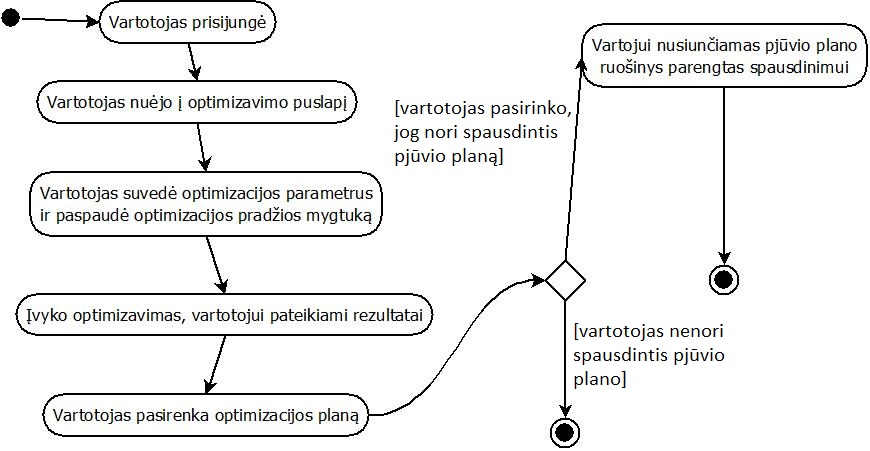
\includegraphics[width=15cm]{swim}


\end{document}
